% Generated by scripts/paper_tables.R in fmegahed/decision-models-for-industrial-image-qc
% from the CSV files in tables/. Do not edit this file: run the script again.
% To use a table, copy it (from \begin{table*} to \end{table*}) into main.tex.
% The captions and the notes are drafts; replace them with your own.
% Table 3 has notes under it and needs \usepackage{threeparttable}. It
% also needs makecell and tikz, and the three macros below (\latx,
% \latglyph and \lataxis): copy them into the preamble of main.tex.
% The description table needs tabularx, xcolor, ulem (normalem) and the
% color jev below.
\documentclass[nohead,nofoot]{asmeconf}
\usepackage{threeparttable,makecell,tikz,tabularx,xcolor}
\usepackage[normalem]{ulem}
\definecolor{jev}{HTML}{00829B}
\newcommand{\latx}[1]{\fpeval{(ln(#1)/ln(10) - 0.69897)*0.38}in}
\newcommand{\latglyph}[5]{\begin{tikzpicture}[baseline=-0.6ex]
  \foreach \t in {10,100,1000} \draw[black!15, line width=0.3pt] (\latx{\t},-3.6pt) -- (\latx{\t},3.6pt);
  \draw[black!55, line width=0.4pt] (\latx{#1},0) -- (\latx{#2},0) (\latx{#4},0) -- (\latx{#5},0);
  \fill[black!25] (\latx{#2},-2.3pt) rectangle (\latx{#4},2.3pt);
  \draw[black, line width=0.9pt] (\latx{#3},-3pt) -- (\latx{#3},3pt);
  \path (0,0) (\latx{2000},0);
\end{tikzpicture}}
\newcommand{\lataxis}{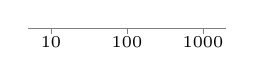
\begin{tikzpicture}[baseline=0pt, font=\fontsize{6}{7}\selectfont]
  \draw[black!50, line width=0.3pt] (0,0) -- (\latx{2000},0);
  \foreach \t in {10,100,1000} {\draw[black!50, line width=0.3pt] (\latx{\t},0) -- (\latx{\t},-2pt);
    \node[anchor=north, inner sep=1pt] at (\latx{\t},-2pt) {\t};}
\end{tikzpicture}}
\begin{document}
\twocolumn % as in the paper (asmeconf starts two columns in \maketitle)
\begin{table*}

\caption{\label{tab:sets}Datasets and sets (images, nominal + defective).}
\centering
\fontsize{8}{10}\selectfont
\begin{tabular}[t]{l>{\raggedright\arraybackslash}p{4.2cm}rrrrr}
\toprule
Dataset & Defect types & Learning set L & References in L ($k = 4$) & Design images & Calibration set C & Test set\\
\midrule
Metallic pans & One defective class & 10 + 10 & 4 + 4 & none (no loop) & none & 39 + 39\\
Extrusion & 2 types: over, under & 50 + 50 & 4 + 4 & 48 + 48 & 25 + 25 & 100 + 100\\
Textiles & 2 types: global, local & 50 + 50 & 4 + 4 & 48 + 48 & 25 + 25 & 100 + 100\\
Pipe staple & Missing staple & 50 + 50 & 4 + 4 & 48 + 48 & 17 + 17 & 50 + 50\\
Microstructure & 9 types: Band, Bimodal, SingleCrystal (low, medium, high) & 50 + 50 & 4 + 4 & 48 + 48 & 25 + 25 & 225 + 225\\
\bottomrule
\end{tabular}
\end{table*}

\begin{table*}

\caption{\label{tab:budget}Label budget: labeled images per class that each method needs ($k = 2$).}
\centering
\fontsize{8}{10}\selectfont
\begin{tabular}[t]{l>{\raggedright\arraybackslash}p{3cm}l>{\centering\arraybackslash}p{2cm}rrrrr}
\toprule
\multicolumn{4}{c}{ } & \multicolumn{5}{c}{Labeled images per class} \\
\cmidrule(l{3pt}r{3pt}){5-9}
Method & Learning & Calibration & Images seen per test image, per class & Metallic pans & Extrusion & Textiles & Pipe staple & Microstructure\\
\midrule
JEV and Clef-Flash & L (k references; the rest chooses the description) & C & k & 10 & 75 & 75 & 67 & 75\\
CLIP baseline & L & C & 50 (pans 10) & 10 & 75 & 75 & 67 & 75\\
CLIP, same references & the k references & C & k & 10 & 27 & 27 & 19 & 27\\
CLIP, zero-shot & none & C & 0 & 10 & 25 & 25 & 17 & 25\\
\bottomrule
\end{tabular}
\end{table*}

\begin{table*}
\caption{Main results on the test sets, after Platt scaling on C: predictive performance, latency, cost and compute. Bold: the best value of each metric on each dataset (the lowest for ECE and Brier); bold does not mark a significant difference (see the paired comparisons).}
\label{tab:main}
\centering\fontsize{8}{10}\selectfont
\begin{threeparttable}
\setlength{\tabcolsep}{3.2pt}
\begin{tabular}{@{}l rrrrrr @{\hspace{14pt}} cr @{\hspace{14pt}} r @{\hspace{14pt}} r@{}}
\toprule
 & \multicolumn{6}{c}{Predictive performance} & \multicolumn{2}{c}{Latency per image (ms)\tnote{a}} & \multicolumn{1}{c}{Cost\tnote{b}} & \multicolumn{1}{c}{Compute\tnote{c}}\\
\cmidrule(r{6pt}){2-7}\cmidrule(lr{6pt}){8-9}\cmidrule(lr{6pt}){10-10}\cmidrule(l){11-11}
Method & Acc. & Sens. & Spec. & AUC & ECE\tnote{\ddag} & Brier & \lataxis & Median & \makecell[r]{USD per\\1,000 images} & \makecell[r]{GPU\\memory (GB)}\\
\midrule
\multicolumn{11}{@{}l}{\textbf{Metallic pans}}\\
\hspace{1em}JEV, $k = 2$ & \textbf{1.000} & \textbf{1.000} & \textbf{1.000} & \textbf{1.000} & \textbf{0.205} & \textbf{0.056} & \latglyph{925.1}{944.4}{969.7}{999.5}{1143.2} & 970 & 0.346 & API \\
\hspace{1em}Clef-Flash, $k = 2$ & 0.885 & 0.769 & \textbf{1.000} & \textbf{1.000} & 0.249 & 0.096 & \latglyph{1159.7}{1183.9}{1211.9}{1243.8}{1301.7} & 1,212 & 0 & 18.8 \\
\hspace{1em}CLIP baseline & 0.641 & 0.282 & \textbf{1.000} & 0.999 & 0.290 & 0.183 & \latglyph{63.2}{65.5}{97.9}{110.9}{136.7} & 98 & 0 & 0.9 \\
\hspace{1em}CLIP, same references, $k = 2$ & 0.744 & 0.487 & \textbf{1.000} & 0.988 & 0.255 & 0.146 & \latglyph{99.7}{107.1}{113.3}{128.1}{143.3} & 113 & 0 & 0.9 \\
\hspace{1em}CLIP, zero-shot & 0.615 & 0.385 & 0.846 & 0.565 & 0.240 & 0.270 & \latglyph{114.2}{118.2}{124.1}{129.3}{146.4} & 124 & 0 & 0.9 \\
\addlinespace[2pt]
\multicolumn{11}{@{}l}{\textbf{Extrusion}}\\
\hspace{1em}JEV, $k = 2$ & \textbf{0.750} & 0.600 & \textbf{0.900} & \textbf{0.826} & 0.134 & 0.193 & \latglyph{152.0}{165.6}{175.1}{195.2}{271.7} & 175 & 0.062 & API \\
\hspace{1em}Clef-Flash, $k = 2$ & 0.710 & 0.580 & 0.840 & 0.799 & 0.091 & \textbf{0.191} & \latglyph{144.3}{167.2}{173.2}{179.9}{188.1} & 173 & 0 & 18.8 \\
\hspace{1em}CLIP baseline & 0.715 & \textbf{0.820} & 0.610 & 0.775 & 0.180 & 0.232 & \latglyph{9.2}{9.7}{10.5}{13.8}{19.0} & 10 & 0 & 0.9 \\
\hspace{1em}CLIP, same references, $k = 2$ & 0.670 & 0.600 & 0.740 & 0.743 & 0.090 & 0.216 & \latglyph{9.0}{10.6}{13.3}{14.7}{15.7} & 13 & 0 & 0.9 \\
\hspace{1em}CLIP, zero-shot & 0.655 & 0.610 & 0.700 & 0.706 & \textbf{0.069} & 0.223 & \latglyph{14.0}{14.8}{15.9}{19.6}{24.2} & 16 & 0 & 0.9 \\
\addlinespace[2pt]
\multicolumn{11}{@{}l}{\textbf{Textiles}}\\
\hspace{1em}JEV, $k = 2$ & 0.965 & 0.930 & \textbf{1.000} & 0.995 & 0.080 & 0.034 & \latglyph{261.9}{276.0}{289.5}{323.4}{456.3} & 290 & 0.062 & API \\
\hspace{1em}Clef-Flash, $k = 2$ & 0.840 & 0.810 & 0.870 & 0.911 & 0.064 & 0.116 & \latglyph{163.0}{186.4}{193.7}{200.7}{229.8} & 194 & 0 & 18.8 \\
\hspace{1em}CLIP baseline & \textbf{0.975} & \textbf{0.970} & 0.980 & \textbf{0.998} & 0.080 & \textbf{0.029} & \latglyph{9.4}{9.8}{10.7}{13.0}{16.1} & 11 & 0 & 0.9 \\
\hspace{1em}CLIP, same references, $k = 2$ & 0.685 & 0.640 & 0.730 & 0.753 & 0.066 & 0.196 & \latglyph{9.3}{9.7}{10.4}{12.9}{16.0} & 10 & 0 & 0.9 \\
\hspace{1em}CLIP, zero-shot\textsuperscript{\dag} & 0.645 & 0.650 & 0.640 & 0.718 & \textbf{0.059} & 0.214 & \latglyph{14.5}{15.2}{16.5}{20.8}{26.0} & 16 & 0 & 0.9 \\
\addlinespace[2pt]
\multicolumn{11}{@{}l}{\textbf{Pipe staple}}\\
\hspace{1em}JEV, $k = 2$ & 0.940 & 0.920 & 0.960 & 0.994 & 0.108 & 0.043 & \latglyph{225.1}{250.3}{269.4}{291.8}{342.2} & 269 & 0.111 & API \\
\hspace{1em}Clef-Flash, $k = 2$ & \textbf{0.990} & \textbf{1.000} & \textbf{0.980} & \textbf{1.000} & 0.108 & \textbf{0.027} & \latglyph{205.7}{249.4}{257.0}{265.8}{287.1} & 257 & 0 & 18.8 \\
\hspace{1em}CLIP baseline & 0.570 & 0.320 & 0.820 & 0.631 & 0.118 & 0.249 & \latglyph{12.4}{12.9}{13.2}{14.2}{16.7} & 13 & 0 & 0.9 \\
\hspace{1em}CLIP, same references, $k = 2$ & 0.670 & 0.680 & 0.660 & 0.686 & \textbf{0.085} & 0.227 & \latglyph{12.3}{12.7}{13.2}{14.1}{18.8} & 13 & 0 & 0.9 \\
\hspace{1em}CLIP, zero-shot & 0.640 & 0.580 & 0.700 & 0.709 & 0.087 & 0.228 & \latglyph{17.2}{17.8}{18.2}{19.0}{21.1} & 18 & 0 & 0.9 \\
\addlinespace[2pt]
\multicolumn{11}{@{}l}{\textbf{Microstructure}}\\
\hspace{1em}JEV, $k = 2$ & 0.902 & 0.822 & \textbf{0.982} & 0.959 & 0.059 & 0.075 & \latglyph{225.0}{242.3}{259.6}{288.9}{404.1} & 260 & 0.114 & API \\
\hspace{1em}Clef-Flash, $k = 2$ & 0.867 & 0.751 & \textbf{0.982} & 0.924 & 0.078 & 0.106 & \latglyph{237.1}{247.1}{257.3}{272.4}{306.9} & 257 & 0 & 18.8 \\
\hspace{1em}CLIP baseline & \textbf{0.933} & \textbf{0.889} & 0.978 & \textbf{0.990} & 0.119 & \textbf{0.061} & \latglyph{10.0}{10.9}{13.2}{15.2}{18.7} & 13 & 0 & 0.9 \\
\hspace{1em}CLIP, same references, $k = 2$ & 0.842 & 0.742 & 0.942 & 0.939 & \textbf{0.057} & 0.106 & \latglyph{9.9}{10.1}{10.3}{10.7}{11.9} & 10 & 0 & 0.9 \\
\hspace{1em}CLIP, zero-shot\textsuperscript{\dag} & 0.640 & 0.667 & 0.613 & 0.688 & 0.101 & 0.235 & \latglyph{15.0}{15.5}{15.9}{16.6}{20.5} & 16 & 0 & 0.9 \\
\bottomrule
\end{tabular}
\begin{tablenotes}[flushleft]\footnotesize
\item[\dag] Negative Platt slope: Platt scaling reverses the order of the raw scores.
\item[\ddag] ECE measures calibration only. Probabilities that stay near 0.5 can reach a low ECE while they separate the classes poorly; their Brier score then stays near 0.25, the score of a constant 0.5 (for example, the lowest ECE on extrusion, textiles and pipe staple). Read ECE with AUC and Brier.
\item[a] Box: Q1 to Q3; whiskers: 5th to 95th percentile; tick and number: median; log scale. JEV: wall time of the call to the TypeSafe API, with the network. Clef-Flash and CLIP: one NVIDIA RTX 5000 Ada Generation GPU; CLIP after one warm-up call, without the one-time encoding of its references (see c).
\item[b] JEV: input tokens times USD 0.042 per million (the output tokens have no price in this estimate). Every JEV call on a dataset had the same number of input tokens, so the standard deviation of the cost per image is 0. Clef-Flash and CLIP run on a local GPU: no cost per image (the hardware and the energy are not counted).
\item[c] GPU memory: the weights of the model. JEV runs on the servers of TypeSafe; its size and hardware are not public, and it needs no local GPU. Each JEV call holds the test image and the $2k$ reference images, so the input tokens per call grow with $k$ (pans: 1,916, 5,092, 8,244 and 14,548 tokens at $k = 0$, 1, 2 and 4), and so does the median time per image (pans: 312 ms at $k = 0$, 1,711 ms at $k = 4$). Clef-Flash is a dense model with 9.41 billion parameters in bfloat16 (2 bytes each): 18.8 GB of weights. On one NVIDIA RTX 5000 Ada Generation, its SGLang server held 24.8 GB, with a reserve for its cache. Like JEV, it reads the references in each call. At about 2 FLOPs per parameter and input token (Kaplan et al., 2020), one test image at $k = 2$ needs $1.2 \times 10^{13}$ to $5.8 \times 10^{13}$ FLOPs, and its median time on pans grows from 294 ms at $k = 0$ to 2,121 ms at $k = 4$. CLIP ViT-L/14 has 0.43 billion parameters, mostly in float16: 0.94 GB of weights on the GPU, and a peak of 0.96 GB while it encodes one image. One test image needs one image encoding ($1.6 \times 10^{11}$ FLOPs) and one comparison with the $n$ stored features of the references, each of 768 numbers ($2 \times 768 \times n$ FLOPs): $1.5 \times 10^{5}$ FLOPs for the baseline ($n = 100$; pans: 20) and $6.1 \times 10^{3}$ FLOPs at $k = 2$ ($n = 4$), about $1 \times 10^{-6}$ of the encoding. CLIP zero-shot also encodes its two prompts for each image ($2.6 \times 10^{10}$ FLOPs). CLIP encodes the references once, before the test images ($n$ encodings: $1.6 \times 10^{13}$ FLOPs for the baseline); the latency does not include this. Thus the latency of CLIP does not grow with $n$ until $n$ is near $1 \times 10^{6}$, where the comparison reaches 1\% of the encoding, while the latency of JEV and Clef-Flash grows with $k$.
\end{tablenotes}
\end{threeparttable}
\end{table*}

\begin{table*}

\caption{\label{tab:paired}Paired comparisons on the test sets: difference (decision model minus the other side) and paired 95\% bootstrap interval. The p-values test the accuracy: McNemar p is the exact McNemar test of the decisions at 0.5, and Holm p adjusts it over the 14 tests of each model. AUC has an interval and no test. A mark on a comparison applies to one of its two sides. \textsuperscript{\dag}Negative Platt slope: Platt scaling reverses the order of the raw scores.}
\centering
\fontsize{8}{10}\selectfont
\begin{tabular}[t]{llrrrr}
\toprule
Comparison & Model & Accuracy & AUC & McNemar p & Holm p\\
\midrule
\addlinespace[0.3em]
\multicolumn{6}{l}{\textbf{Metallic pans}}\\
\hspace{1em}P1 & JEV & +0.359 (0.282 to 0.423) & +0.001 (0.000 to 0.007) & $<$\,0.001 & $<$\,0.001\\
\hspace{1em}P1 & Clef-Flash & +0.244 (0.167 to 0.321) & +0.001 (0.000 to 0.007) & $<$\,0.001 & $<$\,0.001\\
\hspace{1em}P3 & JEV & +0.231 (0.154 to 0.308) & +0.002 (0.000 to 0.008) & $<$\,0.001 & $<$\,0.001\\
\hspace{1em}P3 & Clef-Flash & +0.167 (0.077 to 0.256) & +0.045 (0.004 to 0.098) & 0.002 & 0.016\\
\addlinespace[0.3em]
\multicolumn{6}{l}{\textbf{Extrusion}}\\
\hspace{1em}P1 & JEV & +0.035 ($-$0.035 to 0.115) & +0.052 ($-$0.019 to 0.132) & 0.489 & 1.000\\
\hspace{1em}P1 & Clef-Flash & $-$0.005 ($-$0.080 to 0.075) & +0.024 ($-$0.055 to 0.105) & 1.000 & 1.000\\
\hspace{1em}P2 & JEV & +0.130 (0.070 to 0.190) & +0.112 (0.058 to 0.165) & $<$\,0.001 & $<$\,0.001\\
\hspace{1em}P2 & Clef-Flash & +0.035 ($-$0.020 to 0.090) & +0.002 ($-$0.036 to 0.040) & 0.281 & 0.875\\
\hspace{1em}P3 & JEV & +0.090 (0.040 to 0.145) & +0.068 (0.029 to 0.109) & 0.003 & 0.018\\
\hspace{1em}P3 & Clef-Flash & +0.070 (0.015 to 0.130) & +0.082 (0.045 to 0.121) & 0.029 & 0.173\\
\addlinespace[0.3em]
\multicolumn{6}{l}{\textbf{Textiles}}\\
\hspace{1em}P1 & JEV & $-$0.010 ($-$0.040 to 0.020) & $-$0.002 ($-$0.012 to 0.005) & 0.754 & 1.000\\
\hspace{1em}P1 & Clef-Flash & $-$0.135 ($-$0.190 to $-$0.080) & $-$0.087 ($-$0.131 to $-$0.049) & $<$\,0.001 & $<$\,0.001\\
\hspace{1em}P2 & JEV & +0.145 (0.090 to 0.205) & +0.068 (0.041 to 0.102) & $<$\,0.001 & $<$\,0.001\\
\hspace{1em}P2 & Clef-Flash & +0.085 (0.005 to 0.165) & +0.046 ($-$0.023 to 0.116) & 0.057 & 0.284\\
\hspace{1em}P3 & JEV & +0.090 (0.050 to 0.135) & +0.021 (0.004 to 0.039) & $<$\,0.001 & $<$\,0.001\\
\hspace{1em}P3 & Clef-Flash & +0.145 (0.095 to 0.200) & +0.119 (0.082 to 0.160) & $<$\,0.001 & $<$\,0.001\\
\addlinespace[0.3em]
\multicolumn{6}{l}{\textbf{Pipe staple}}\\
\hspace{1em}P1 & JEV & +0.370 (0.280 to 0.470) & +0.364 (0.257 to 0.477) & $<$\,0.001 & $<$\,0.001\\
\hspace{1em}P1 & Clef-Flash & +0.420 (0.340 to 0.500) & +0.369 (0.263 to 0.482) & $<$\,0.001 & $<$\,0.001\\
\hspace{1em}P2 & JEV & 0.000 ($-$0.030 to 0.030) & +0.001 ($-$0.003 to 0.005) & 1.000 & 1.000\\
\hspace{1em}P2\textsuperscript{\dag} & Clef-Flash & +0.530 (0.430 to 0.620) & +0.519 (0.400 to 0.629) & $<$\,0.001 & $<$\,0.001\\
\hspace{1em}P3\textsuperscript{\dag} & JEV & +0.210 (0.110 to 0.310) & +0.185 (0.106 to 0.273) & $<$\,0.001 & 0.001\\
\hspace{1em}P3 & Clef-Flash & +0.040 (0.000 to 0.090) & +0.035 (0.006 to 0.075) & 0.219 & 0.875\\
\addlinespace[0.3em]
\multicolumn{6}{l}{\textbf{Microstructure}}\\
\hspace{1em}P1 & JEV & $-$0.031 ($-$0.058 to $-$0.004) & $-$0.031 ($-$0.050 to $-$0.015) & 0.034 & 0.168\\
\hspace{1em}P1 & Clef-Flash & $-$0.067 ($-$0.098 to $-$0.036) & $-$0.066 ($-$0.093 to $-$0.042) & $<$\,0.001 & $<$\,0.001\\
\hspace{1em}P2 & JEV & +0.147 (0.107 to 0.187) & +0.120 (0.087 to 0.157) & $<$\,0.001 & $<$\,0.001\\
\hspace{1em}P2 & Clef-Flash & +0.064 (0.033 to 0.096) & +0.016 ($-$0.011 to 0.043) & $<$\,0.001 & 0.002\\
\hspace{1em}P3 & JEV & +0.013 ($-$0.009 to 0.036) & +0.025 (0.012 to 0.039) & 0.362 & 1.000\\
\hspace{1em}P3 & Clef-Flash & +0.013 ($-$0.009 to 0.036) & +0.041 (0.023 to 0.060) & 0.362 & 0.875\\
\bottomrule
\end{tabular}
\end{table*}

\begin{table*}

\caption{\label{tab:calibration}Calibration on the test sets, before (raw) and after Platt scaling on C. \textsuperscript{\dag}Negative Platt slope: Platt scaling reverses the order of the raw scores.}
\centering
\fontsize{8}{10}\selectfont
\begin{tabular}[t]{lrrrr}
\toprule
\multicolumn{1}{c}{ } & \multicolumn{2}{c}{ECE} & \multicolumn{2}{c}{Brier} \\
\cmidrule(l{3pt}r{3pt}){2-3} \cmidrule(l{3pt}r{3pt}){4-5}
Method & Raw & Platt & Raw & Platt\\
\midrule
\addlinespace[0.3em]
\multicolumn{5}{l}{\textbf{Metallic pans}}\\
\hspace{1em}JEV, $k = 2$ & 0.114 & 0.205 & 0.016 & 0.056\\
\hspace{1em}Clef-Flash, $k = 2$ & 0.211 & 0.249 & 0.140 & 0.096\\
\hspace{1em}CLIP baseline & 0.407 & 0.290 & 0.247 & 0.183\\
\hspace{1em}CLIP, same references, $k = 2$ & 0.131 & 0.255 & 0.245 & 0.146\\
\hspace{1em}CLIP, zero-shot & 0.182 & 0.240 & 0.250 & 0.270\\
\addlinespace[0.3em]
\multicolumn{5}{l}{\textbf{Extrusion}}\\
\hspace{1em}JEV, $k = 2$ & 0.115 & 0.134 & 0.181 & 0.193\\
\hspace{1em}Clef-Flash, $k = 2$ & 0.085 & 0.091 & 0.194 & 0.191\\
\hspace{1em}CLIP baseline & 0.191 & 0.180 & 0.248 & 0.232\\
\hspace{1em}CLIP, same references, $k = 2$ & 0.120 & 0.090 & 0.246 & 0.216\\
\hspace{1em}CLIP, zero-shot & 0.085 & 0.069 & 0.227 & 0.223\\
\addlinespace[0.3em]
\multicolumn{5}{l}{\textbf{Textiles}}\\
\hspace{1em}JEV, $k = 2$ & 0.204 & 0.080 & 0.065 & 0.034\\
\hspace{1em}Clef-Flash, $k = 2$ & 0.214 & 0.064 & 0.195 & 0.116\\
\hspace{1em}CLIP baseline & 0.473 & 0.080 & 0.248 & 0.029\\
\hspace{1em}CLIP, same references, $k = 2$ & 0.188 & 0.066 & 0.249 & 0.196\\
\hspace{1em}CLIP, zero-shot\textsuperscript{\dag} & 0.423 & 0.059 & 0.443 & 0.214\\
\addlinespace[0.3em]
\multicolumn{5}{l}{\textbf{Pipe staple}}\\
\hspace{1em}JEV, $k = 2$ & 0.284 & 0.108 & 0.125 & 0.043\\
\hspace{1em}Clef-Flash, $k = 2$ & 0.346 & 0.108 & 0.173 & 0.027\\
\hspace{1em}CLIP baseline & 0.069 & 0.118 & 0.250 & 0.249\\
\hspace{1em}CLIP, same references, $k = 2$ & 0.169 & 0.085 & 0.250 & 0.227\\
\hspace{1em}CLIP, zero-shot & 0.407 & 0.087 & 0.405 & 0.228\\
\addlinespace[0.3em]
\multicolumn{5}{l}{\textbf{Microstructure}}\\
\hspace{1em}JEV, $k = 2$ & 0.142 & 0.059 & 0.123 & 0.075\\
\hspace{1em}Clef-Flash, $k = 2$ & 0.290 & 0.078 & 0.262 & 0.106\\
\hspace{1em}CLIP baseline & 0.334 & 0.119 & 0.248 & 0.061\\
\hspace{1em}CLIP, same references, $k = 2$ & 0.223 & 0.057 & 0.248 & 0.106\\
\hspace{1em}CLIP, zero-shot\textsuperscript{\dag} & 0.181 & 0.101 & 0.273 & 0.235\\
\bottomrule
\end{tabular}
\end{table*}

\begin{table}
\centering
\caption{\label{tab:prevalence}Precision at lower defect rates, from the test sensitivity and specificity after Platt scaling on C (decision at 0.5), if the scores of each class keep their distribution. \textsuperscript{\dag}Negative Platt slope: Platt scaling reverses the order of the raw scores.}
\centering
\fontsize{8}{10}\selectfont
\begin{tabular}[t]{lrrr}
\toprule
\multicolumn{1}{c}{ } & \multicolumn{3}{c}{Defect rate} \\
\cmidrule(l{3pt}r{3pt}){2-4}
Method & 50\% & 5\% & 1\%\\
\midrule
\addlinespace[0.3em]
\multicolumn{4}{l}{\textbf{Metallic pans}}\\
\hspace{1em}JEV, $k = 2$ & 1.000 & 1.000 & \vphantom{1} 1.000\\
\hspace{1em}Clef-Flash, $k = 2$ & 1.000 & 1.000 & 1.000\\
\hspace{1em}CLIP baseline & 1.000 & 1.000 & 1.000\\
\hspace{1em}CLIP, same references, $k = 2$ & 1.000 & 1.000 & 1.000\\
\hspace{1em}CLIP, zero-shot & 0.714 & 0.116 & 0.025\\
\addlinespace[0.3em]
\multicolumn{4}{l}{\textbf{Extrusion}}\\
\hspace{1em}JEV, $k = 2$ & 0.857 & 0.240 & 0.057\\
\hspace{1em}Clef-Flash, $k = 2$ & 0.784 & 0.160 & 0.035\\
\hspace{1em}CLIP baseline & 0.678 & 0.100 & 0.021\\
\hspace{1em}CLIP, same references, $k = 2$ & 0.698 & 0.108 & 0.023\\
\hspace{1em}CLIP, zero-shot & 0.670 & 0.097 & 0.020\\
\addlinespace[0.3em]
\multicolumn{4}{l}{\textbf{Textiles}}\\
\hspace{1em}JEV, $k = 2$ & 1.000 & 1.000 & 1.000\\
\hspace{1em}Clef-Flash, $k = 2$ & 0.862 & 0.247 & 0.059\\
\hspace{1em}CLIP baseline & 0.980 & 0.719 & 0.329\\
\hspace{1em}CLIP, same references, $k = 2$ & 0.703 & 0.111 & 0.023\\
\hspace{1em}CLIP, zero-shot\textsuperscript{\dag} & 0.644 & 0.087 & 0.018\\
\addlinespace[0.3em]
\multicolumn{4}{l}{\textbf{Pipe staple}}\\
\hspace{1em}JEV, $k = 2$ & 0.958 & 0.548 & 0.189\\
\hspace{1em}Clef-Flash, $k = 2$ & 0.980 & 0.725 & 0.336\\
\hspace{1em}CLIP baseline & 0.640 & 0.086 & 0.018\\
\hspace{1em}CLIP, same references, $k = 2$ & 0.667 & 0.095 & 0.020\\
\hspace{1em}CLIP, zero-shot & 0.659 & 0.092 & 0.019\\
\addlinespace[0.3em]
\multicolumn{4}{l}{\textbf{Microstructure}}\\
\hspace{1em}JEV, $k = 2$ & 0.979 & 0.709 & 0.318\\
\hspace{1em}Clef-Flash, $k = 2$ & 0.977 & 0.690 & 0.299\\
\hspace{1em}CLIP baseline & 0.976 & 0.678 & 0.288\\
\hspace{1em}CLIP, same references, $k = 2$ & 0.928 & 0.403 & 0.115\\
\hspace{1em}CLIP, zero-shot\textsuperscript{\dag} & 0.633 & 0.083 & 0.017\\
\bottomrule
\end{tabular}
\end{table}

\begin{table*}
\caption{\label{tab:description-wide}The descriptions that the JEV description loop kept for extrusion.}
\centering
\fontsize{8}{10}\selectfont
\begin{threeparttable}
\begin{tabularx}{\textwidth}{@{}cc>{\raggedright\arraybackslash}X>{\raggedright\arraybackslash}X@{}}
\toprule
Candidate & Design AUC & Nominal description & Defective description \\
\midrule
1 & 0.59 & No visible manufacturing defects; the part appears conforming. & At least one visible manufacturing defect or anomaly. \\
2 & 0.74 & A close-up of a 3D printing nozzle and freshly extruded plastic; the extruded material forms a smooth, even layer of steady width that lies flat on the print surface.\textsuperscript{\dag} & A close-up of a 3D printing nozzle and extruded plastic where the amount of material is wrong: either a thin, stringy or broken strand with dark gaps showing through, or a bulging, blobby, overly wide mass of plastic.\textsuperscript{\dag} \\
3 & 0.78 & A close-up of a 3D printing nozzle and freshly extruded plastic; the extruded material forms a smooth, even layer \textcolor{jev}{\textbf{or strand}} of steady width \textcolor{black!60}{\sout{that lies flat on the print surface.}} \textcolor{jev}{\textbf{with straight, clean edges. The background around it may be dark or light.}} & A close-up of a 3D printing nozzle and extruded plastic where the amount of material is wrong: either a thin, stringy \textcolor{black!60}{\sout{or broken strand with dark gaps showing through,}} \textcolor{jev}{\textbf{strand with breaks or gaps within the plastic itself,}} or a bulging, blobby, overly wide mass of plastic. \\
\bottomrule
\end{tabularx}
\begin{tablenotes}[flushleft]\footnotesize\raggedright
\item Each text is shown against the text it revised: added words in color and bold, removed words struck through. Design AUC: on the design set of the loop. \textsuperscript{\dag}Written anew (keeps less than a quarter of the words of the text it revised).
\item The instructions of the loop agent (\texttt{LOOP.md}; its prompt is ``Read LOOP.md and follow it.''), on how to make a change: ``Read the printed result: the AUC, the mean score for each defect type and the current best candidate. Open \texttt{scores/N.csv} to see which images get the wrong scores.'' \ldots\ ``Look at the images that the model ranks wrongly. Compare them with the reference images.'' \ldots\ ``Base each change on what you see in the design images and in the scores. Change one idea at a time, so that the log shows what helped.'' \ldots\ ``Do not aim for an AUC of 1. A small design set can mislead you. Prefer a clear, general description over a long list of special cases.'' (\texttt{scripts/fair\_loop\_instructions.md}).
\item All eight loops, with the candidates that the loops did not keep: \url{https://fmegahed.github.io/decision-models-for-industrial-image-qc/pages/description_loops.html}.
\end{tablenotes}
\end{threeparttable}
\end{table*}

\begin{table}
\caption{\label{tab:description-long}The descriptions that the JEV description loop kept for extrusion.}
\centering
\fontsize{8}{10}\selectfont
\begin{threeparttable}
\begin{tabularx}{\columnwidth}{@{}l>{\raggedright\arraybackslash}X@{}}
\toprule
\multicolumn{2}{@{}l}{\textbf{Candidate 1}, design AUC 0.59} \\
Nominal & No visible manufacturing defects; the part appears conforming. \\
Defective & At least one visible manufacturing defect or anomaly. \\
\addlinespace
\multicolumn{2}{@{}l}{\textbf{Candidate 2}, design AUC 0.74} \\
Nominal & A close-up of a 3D printing nozzle and freshly extruded plastic; the extruded material forms a smooth, even layer of steady width that lies flat on the print surface.\textsuperscript{\dag} \\
Defective & A close-up of a 3D printing nozzle and extruded plastic where the amount of material is wrong: either a thin, stringy or broken strand with dark gaps showing through, or a bulging, blobby, overly wide mass of plastic.\textsuperscript{\dag} \\
\addlinespace
\multicolumn{2}{@{}l}{\textbf{Candidate 3}, design AUC 0.78} \\
Nominal & A close-up of a 3D printing nozzle and freshly extruded plastic; the extruded material forms a smooth, even layer \textcolor{jev}{\textbf{or strand}} of steady width \textcolor{black!60}{\sout{that lies flat on the print surface.}} \textcolor{jev}{\textbf{with straight, clean edges. The background around it may be dark or light.}} \\
Defective & A close-up of a 3D printing nozzle and extruded plastic where the amount of material is wrong: either a thin, stringy \textcolor{black!60}{\sout{or broken strand with dark gaps showing through,}} \textcolor{jev}{\textbf{strand with breaks or gaps within the plastic itself,}} or a bulging, blobby, overly wide mass of plastic. \\
\bottomrule
\end{tabularx}
\begin{tablenotes}[flushleft]\footnotesize\raggedright
\item Each text is shown against the text it revised: added words in color and bold, removed words struck through. Design AUC: on the design set of the loop. \textsuperscript{\dag}Written anew (keeps less than a quarter of the words of the text it revised).
\item The instructions of the loop agent (\texttt{LOOP.md}; its prompt is ``Read LOOP.md and follow it.''), on how to make a change: ``Read the printed result: the AUC, the mean score for each defect type and the current best candidate. Open \texttt{scores/N.csv} to see which images get the wrong scores.'' \ldots\ ``Look at the images that the model ranks wrongly. Compare them with the reference images.'' \ldots\ ``Base each change on what you see in the design images and in the scores. Change one idea at a time, so that the log shows what helped.'' \ldots\ ``Do not aim for an AUC of 1. A small design set can mislead you. Prefer a clear, general description over a long list of special cases.'' (\texttt{scripts/fair\_loop\_instructions.md}).
\item All eight loops, with the candidates that the loops did not keep: \url{https://fmegahed.github.io/decision-models-for-industrial-image-qc/pages/description_loops.html}.
\end{tablenotes}
\end{threeparttable}
\end{table}

\end{document}
